\documentclass[11pt]{ctexbeamer}
\usetheme{Darmstadt}
\usepackage{amsmath}
\usepackage{amsfonts}
\usepackage{amssymb}
\usepackage{graphics}
\usepackage{color}
\addtobeamertemplate{block begin}{%
  \setlength{\textwidth}{0.9\textwidth}%
}{}

\addtobeamertemplate{block alerted begin}{%
  \setlength{\textwidth}{0.9\textwidth}%
}{}

\addtobeamertemplate{block example begin}{%
  \setlength{\textwidth}{0.9\textwidth}%
}{}
\author{周亮}
\title{近期工作总结}
\graphicspath{{fig/}}
%\setbeamercovered{transparent}
%\setbeamertemplate{navigation symbols}{}
\logo{
\includegraphics[scale=0.1]{icons_nudt.jpg}}
\institute{102教研室}
\date{\today}
%\subject{}
\begin{document}

\begin{frame}
	\titlepage
\end{frame}

\begin{frame}
	\tableofcontents
\end{frame}

\section{月地转移轨道设计}
\subsection{双二体假设下计算模型}

\subsection{瞄准参数分析}
\begin{frame}{再入可达域分析工作}
	\begin{minipage}{0.4\linewidth}
		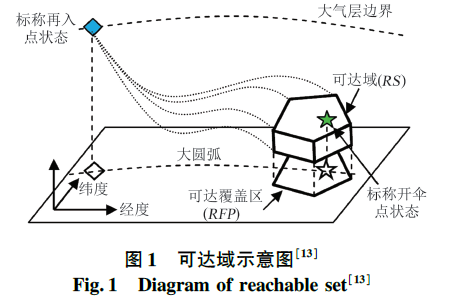
\includegraphics[height=.4\textheight]{reachable_set.png}
	\end{minipage}
	\hspace{1cm}
	\begin{minipage}{0.4\linewidth}
		\begin{block}{求解思路}
			\begin{enumerate}
				\item 优化计算沿初始速度方向纵程的最小值和最大值;
				\item 在纵程范围选取一系列离散点,在这些点上优化计算横程的最小值和最大值(对应横程符号一正一负)
			\end{enumerate}
		\end{block}
	\end{minipage}
	\begin{block}{参考书目}
		\begin{itemize}
			\item {{\color{red} 探月飞船跳跃式再入轨迹可达域分析}[J],杜昕}
			\item Gauss伪谱法的再入可达域计算方法[J],王涛\\
			      滑翔飞行器,换极坐标系下求解可达域。
		\end{itemize}
	\end{block}
\end{frame}
\begin{frame}{再入可达域设计结果}
	模型:未考虑自转、圆球假设,固定初始状态

	约束:热流、过载、动压均设置
	\begin{block}{设计结果}
		最大航程:1.0466e+07    1.6427\\
		最小航程:1.6336e+06    0.2564\\
		横程范围:400-700km左右\\
		\begin{minipage}{0.4\linewidth}
			\centering
			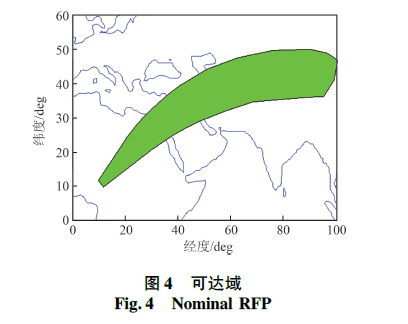
\includegraphics[height=.4\textheight]{nominal_RFP.png}
		\end{minipage}
		\hspace{1cm}
		\begin{minipage}{0.4\linewidth}
			\centering
			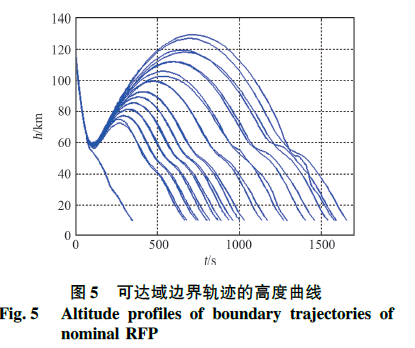
\includegraphics[height=.4\textheight]{RFP_altitude_profile.png}
		\end{minipage}
	\end{block}
\end{frame}
\begin{frame}{再入可达域设计问题}
	得到航程范围后的过程与邹毅论文中方法不一致。(原方法的航程调节范围很小,相对地球半径是小量)。\\
	\begin{figure}[]
		\centering
		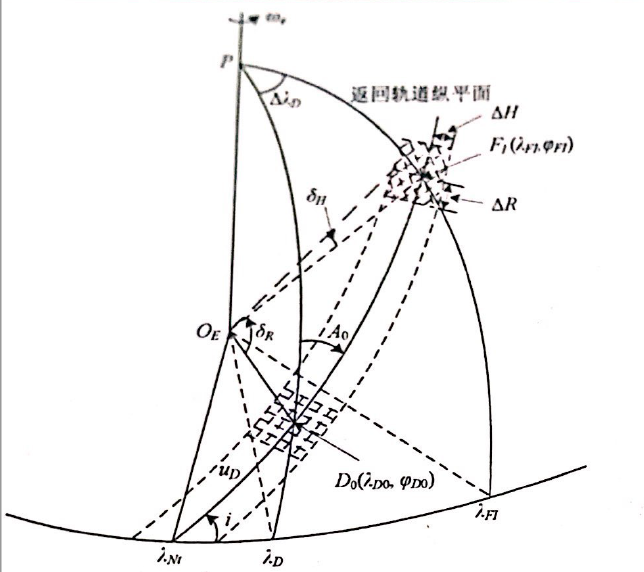
\includegraphics[height=.6\textheight]{old_method.png}
		\caption{原论文中的返回航程可调示意图}
	\end{figure}
\end{frame}
\begin{frame}{再入可达域设计问题}
	气动系数的插值,导致伪谱程序求解慢,效率差10倍左右\\
	能否采用拟合的方式\\
	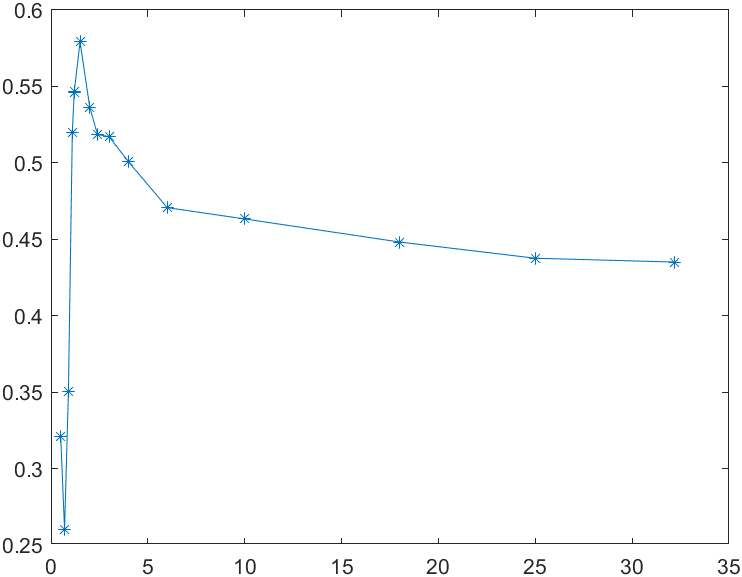
\includegraphics[height=.4\textheight]{Ma_Cl.png}
	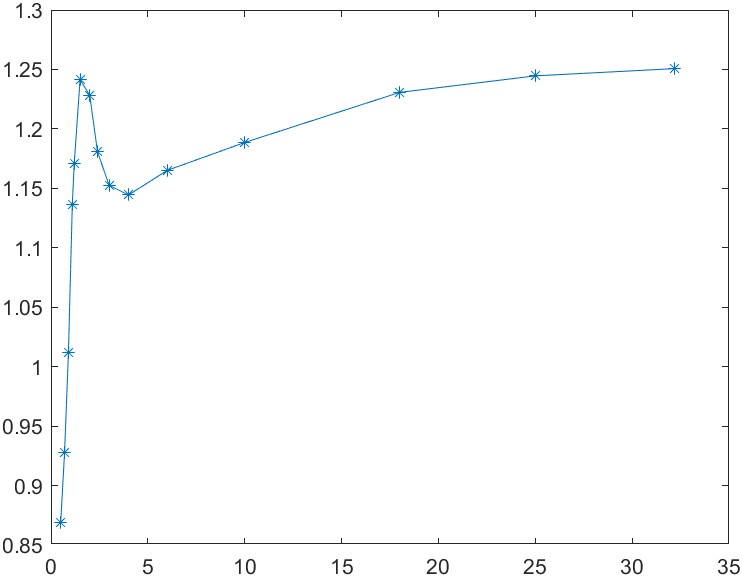
\includegraphics[height=.4\textheight]{Ma_Cd.png}

\end{frame}
\begin{frame}{再入可达域设计问题}
	\begin{block}{可能的思路}
		问题的关键是获得再入点处的范围,即返回轨道的瞄准参数,利用简化模型,不考虑自转等其他因素。\\
		因为落场是固定的,(原问题固定初始点的假设可能不再成立),可以考虑固定终端,初始再入点的经纬度作为优化量,优化求解。
	\end{block}
\end{frame}
\section{下周计划}
\begin{frame}{工作计划}
	\begin{block}{}
		\begin{enumerate}
			\item 明确采用什么模型进行空间轨道设计与再入轨道设计,(双二体模型或者考虑摄动的精确模型)
			\item 确定再入瞄准点的选择方法(是否考虑其中的黄金再入走廊等方式)
			\item 完成再入可达域的绘图分析部分
		\end{enumerate}
	\end{block}
\end{frame}
\end{document}